\section{Parallel I/O}

Input-output could be a serious bottleneck if we do not pay the right attention.
In particular, when dealing with supercomputers, two major problems arise:
\begin{itemize}
\item needing of parallel I/O,
\item avoid endianness problem related.
\end{itemize}
As first thing let us introduce I/O.\par
In computer architecture, the combination of the CPU and main memory, to which the CPU can read or write directly using individual instructions, is considered the brain of a computer. Any transfer of information to or from the CPU/memory combo, for example by reading data from a disk drive, is considered I/O~\cite{io}.
When dealing with cluster the transit of data from disk to CPU is not so straightforward. The presence of multiple CPU require the adoption of one of the following strategies.\par
\begin{wrapfloat}{figure}{l}{0pt}
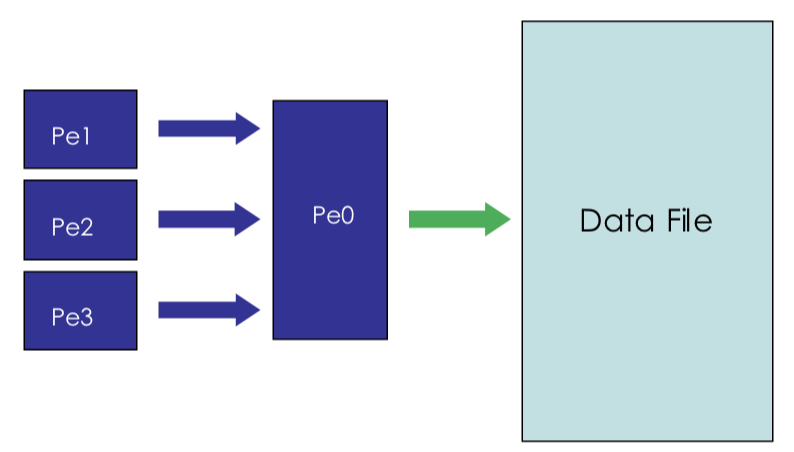
\includegraphics[width=0.5\textwidth]{grafici/masterslave}
\caption{Master-Slaves I/O setup}
\end{wrapfloat}
The most basic strategy is called ``Master-Slave''. In this kind of strategy a single node of the grid have access to the storage, therefore no scalability is provided. The slave nodes must send/receive data from the master, therefore we face strong slowdown related to the huge workload required to perform I/O by the single node and the following communications among nodes.\\

\begin{wrapfloat}{figure}{r}{0pt}
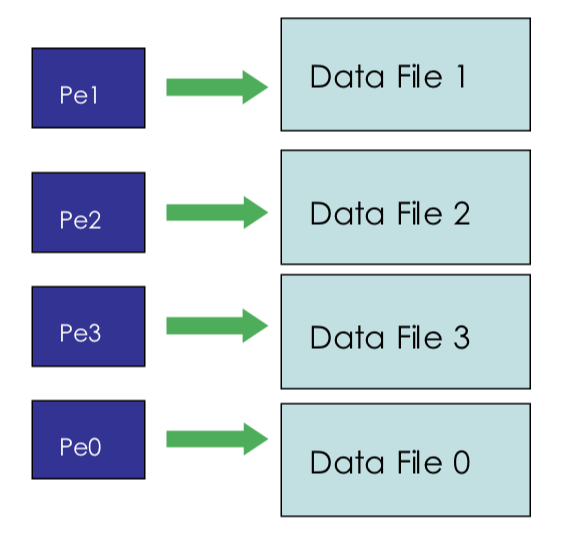
\includegraphics[width=0.5\textwidth]{grafici/localio}
\caption{Distributed I/O on local files}
\end{wrapfloat}
\par
The setup shown here beside perform distributed I/O on local files. Such kind of implementation is scalable, ensure data consistency and avoid communication during I/O phase. However, since every processor writes data on its own hard storage, it require a great deal of post processing work to glue data among each others, which increase linearly with the number of nodes. For this reason we can not consider it affordable. \\

\begin{wrapfloat}{figure}{r}{0pt}
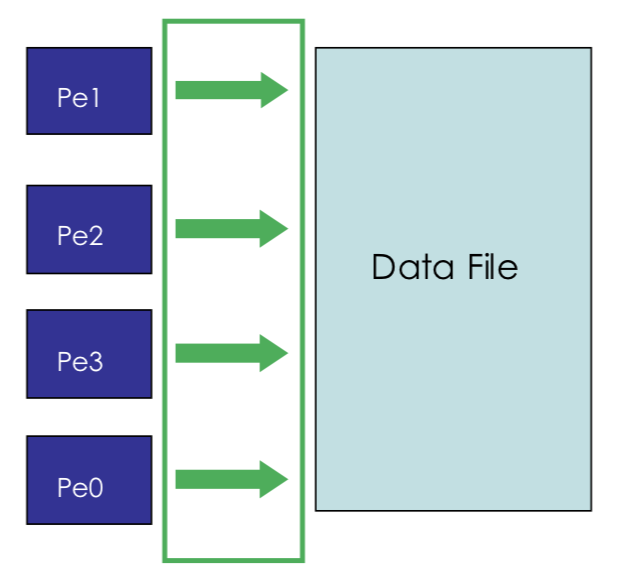
\includegraphics[width=0.5\textwidth]{grafici/mpiio}
\caption{Coordinated controlled accesses}
\end{wrapfloat}
\par
The last kind of I/O setup, which is the most updated and optimized, is the so called coordinated controlled accesses.
Scalability reaches its peak with this kind of implementation, which takes care of possible communications needing by its own.
In this approach every CPU can access to the single storage memory in which the dataset is hosted, and in concomitancy with the other processes, writes the data. As can be understood, the reading/writing operation is intrinsically fragile, since guarantee data consistency can be hard. To avoid consistency lacks, the MPI-IO has been introduced with the deployment of MPI-2 standard~\cite{MPI:standard2}.

On top of MPI-IO different high level I/O libraries arose, two well established examples are parallel netCDF, and HDF5. 

At exception of the ``Master-Slave'' approach, every presented strategy require the adoption of a parallel File System.

Let us establish the concept of endianness.
Intel introduces their white paper with the following sentence:\par
``Endianness describes how multi-byte data is represented by a computer system and is dictated by the CPU architecture of the system. Unfortunately not all computer systems are designed with the same Endian-architecture. The difference in Endian-architecture is an issue when software or data is shared between computer systems''\cite{endianness}.\par
Since our database has been built on Marconi, at Cineca, but the post-processing analysis take place on our personal computers, we need a reliable method to store the data. 

Most computer systems prefer a single format for all their data; using the system's native format is automatic. But when reading memory or receiving transmitted data from a different computer system, it is often required to process and translate data between the preferred native endianness format to the opposite format.